\documentclass[12pt,a4paper]{article}
\usepackage[utf8]{inputenc}
\usepackage[ngerman]{babel}
\usepackage[T1]{fontenc}

% Hauptdatei des Projektes. Von hier aus werden die anderen Seiten eingebunden
\usepackage{amsmath}
\usepackage{amsfonts}
\usepackage{amssymb}
\usepackage{xspace}
\usepackage[normalem]{ulem}
\usepackage{graphicx}
\usepackage{color}

%Schriftart

\renewcommand*\rmdefault{cmdh}
\usepackage{lmodern}
%\usepackage{mathptmx}
%\usepackage[scaled=.90]{helvet}
%\usepackage{courier}
%\usepackage{bera}
%\usepackage{boisik}


%%%%%%%%%%%%%%%%%%%%%%%%%%%%%%%%%%%%%%%%%%%%%%%%%%%%%%%%%%%%%%%%%%%%%%%%%%%%%%%%%%%%%%%%%%
% In diesem Abschnitt gibst du deine persönlichen Daten sowie den Kontext deiner Arbeit an
% das \xspace am Ende der Einträge muss vorhanden bleiben. Es regelt das Whitespace-
% handling
%%%%%%%%%%%%%%%%%%%%%%%%%%%%%%%%%%%%%%%%%%%%%%%%%%%%%%%%%%%%%%%%%%%%%%%%%%%%%%%%%%%%%%%%%%
% persönliche Daten
\newcommand{\beteiligte}{Achim Rose, Tim Wieder, Sebastian Seeger\xspace}
\newcommand{\emailadresse}{achim.rose@et.hs-fulda.de\\tim.wieder@et.hs-fulda.de\\sebastian.seeger@et.hs-fulda.de\xspace}
%\newcommand{\matrikelnummer}{541608\xspace}

% Arbeitsspezifische Daten
\newcommand{\project}{\textbf{WBS ALARM!} (\textit{Arbeitstitel})}
\newcommand{\titel}{\project\xspace}
\newcommand{\untertitel}{IT-Projekt im Rahmen des Studiengangs\xspace}
\newcommand{\modulname}{IT-Projekt\xspace}
\newcommand{\pruefer}{Uwe Werner\xspace}
\newcommand{\semester}{WiSe 18/19 - SoSe 2020\xspace}
\newcommand{\ortderarbeit}{Kassel\xspace}
%%%%%%%%%%%%%%%%%%%%%%%%%%%%%%%%%%%%%%%%%%%%%%%%%%%%%%%%%%%%%%%%%%%%%%%%%%%%%%%%%%%%%%%%%%

%Um einzelne Seite im Querformat zu verwenden
\usepackage{pdflscape}


%Hurenkinder uns Schusterjungen
\clubpenalty10000
\widowpenalty10000
\displaywidowpenalty=10000

\usepackage{hyperxmp} % XMP-Daten fuer die PDF-Datei
%Gimmmick: Linked Kapitel und Inhaltsverzeichnis, sowie Referenzen
\usepackage[pdftex, pdfa]{hyperref}
\hypersetup{
    colorlinks,
    citecolor=black,
    filecolor=black,
    linkcolor=black,
    urlcolor=black,    
    pdftitle = {\titel},
    pdfauthor = {\beteiligte},
    pdfsubject = {\untertitel},
    pdfkeywords = {\titel \untertitel},
    pdflang = de,
    bookmarks = true,
    pdfdisplaydoctitle = true,
    colorlinks = true,
    plainpages = false,
    %allcolors = black,
    hypertexnames = false,
    pdfpagelabels = true,
    hyperindex = true,
    unicode = true,
    pdfcaptionwriter = {\textsl{\beteiligte}},
    pdfcontactaddress = {},
    pdfcontactcity = {Kassel},
    pdfcontactpostcode = {34119},
    pdfcontactcountry = {Deutschland},
    pdfcontactregion = {Hessen},
    pdfcontactemail = {\emailadresse},
    pdfcontactphone = {},
    pdfcontacturl = {http://www.hs-fulda.de},
    pdfmetalang = {de},
}

\usepackage{prettyref}
\usepackage{titleref}


%Inhaltsverzeichnis
\usepackage[tocgraduated]{tocstyle}
\usetocstyle{allwithdot}
\setcounter{tocdepth}{3}

% Formatierungshilfen: http://wwws.htwk-leipzig.de/~myagovki/latex/formatierungshilfen/

\usepackage[ddmmyyyy]{datetime}
\renewcommand{\dateseparator}{.}

% Für Kopf und Fußzeile: https://esc-now.de/_/latex-individuelle-kopf--und-fusszeilen/?lang=en
\usepackage[
  headsepline, plainheadsepline,
  footsepline, plainfootsepline
]{scrlayer-scrpage}
\pagestyle{scrheadings}
\clearscrheadfoot

\ihead*{\titel}
%\ohead*{\vorname \nachname}
\ifoot*{\today}
\ofoot*{\pagemark}

% anderthalbfacher Zeilenabstand
\usepackage[onehalfspacing]{setspace}

%Geometry der Seite festlegen
\usepackage{geometry}
\geometry{
  left=2.5cm,
  right=2.5cm,
  top=2.5cm,
  bottom=2.5cm,
  headheight=33pt
}

%Für Gestaltung des Layouts
\usepackage{blindtext}

%Bilbliothek und Literatur einbinden
\usepackage[style=authoryear-ibid,natbib=true,backend=biber,sorting=nty]{biblatex}
\usepackage[babel,german=guillemets]{csquotes}
\defbibheading{head}{{\section*{Literaturverzeichnis}\addcontentsline{toc}{section}{Literaturverzeichnis}}}
\addbibresource{bib/literatur.bib}

\newcommand{\zb}{z.\,B.\xspace}
\newcommand{\ua}{u.\,a.\xspace}
\newcommand{\oge}{o.\,g.\xspace}
\newcommand{\dah}{d.\,h.\xspace}
\newcommand{\bzw}{bzw.\xspace}
\newcommand{\bzgl}{bzgl.\xspace}

%https://stackoverflow.com/questions/3175105/writing-code-in-latex-document
\newcommand{\code}[1]{\texttt{#1}}

%https://tex.stackexchange.com/questions/115467/listings-highlight-java-annotations
\usepackage{listings}
\usepackage{inconsolata}

\definecolor{pblue}{rgb}{0.13,0.13,1}
\definecolor{pgreen}{rgb}{0,0.5,0}
\definecolor{pgrey}{rgb}{0.46,0.45,0.48}
\definecolor{mauve}{rgb}{0.58,0,0.82}

\usepackage{listings}

\lstset{
  frame=t,
  language=Java,
  aboveskip=1mm,
  belowskip=1mm,
  columns=flexible,
  showspaces=false,
  showtabs=false,
  numbers=left,
  breaklines=true,
  showstringspaces=false,
  breakatwhitespace=true,
  commentstyle=\color{pgreen},
  keywordstyle=\color{pblue},
  stringstyle=\color{mauve},
  basicstyle={\small\ttfamily},
  breaklines=true,
  breakatwhitespace=true,
  tabsize=2,
  moredelim=[il][\textcolor{pgrey}]{$$}, %$$ 
  moredelim=[is][\textcolor{pgrey}]{\%\%}{\%\%}
}

% Silbentrennung
\hyphenation{Funk-tions-be-reich}
\hyphenation{An-wen-der-be-tre-uung}



%https://www.dante.de/events/dante2015/Programm/vortraege/vortrage-partosch2.pdf


\immediate\pdfobj stream attr{/N 3} file{res/AdobeRGB1998.icc}
\pdfcatalog{%
/OutputIntents [ <<
/Type /OutputIntent
/S/GTS_PDFA1
/DestOutputProfile \the\pdflastobj\space 0 R
/OutputConditionIdentifier (Adobe RGB 1998)
/Info(Adobe RGB 1998)
>> ]
}

\input{glyphtounicode.tex}
\input{glyphtounicode-cmr.tex}
\pdfgentounicode=1
\pdfobjcompresslevel=0
\pdfinclusioncopyfonts=1


\begin{document}

%!TEX root = ../hausarbeit.tex
\begin{titlepage}
\newgeometry{
  left=2.5cm,
  right=2.5cm,
  top=2.5cm,
  bottom=2cm
}
\begin{figure}
  \centering
  
\includegraphics[width=1.0\textwidth]{res/hs_fulda_logo.png}
%   \caption{Meine Abbildung}
%   \label{fig:mein-bild}
\end{figure}
    \centering
    Hochschule Fulda \\    Fachbereich Elektrotechnik
    \vspace{1.5cm}

    {\Huge \bfseries \titel \par}
    {\Large \itshape \untertitel \par}
    \vspace{2.5cm}

    Handout zum Vortag\\ im Modul
    %Schriftliche Prüfungsleistung\\ im Modul
    \modulname\\
    im Studiengang\\ Bachelor of Science: Sozialinformatik \\
    \vspace{0.7cm}

    \semester\\

    \vspace{3cm}
    Prüfer: \pruefer\\

    \vfill

% Bottom of the page
    vorgelegt von \\ \beteiligte \\ \emailadresse 
\restoregeometry
\end{titlepage}


\pagenumbering{roman}
\setcounter{page}{2}

\tableofcontents

\newpage

\pagenumbering{arabic}

% Abstand nach Absätzen
\setlength{\parskip}{0.3cm}

% hier wird die Datei mit dem eigentlichen Inhalt der Hausarbeit eingebunden
\section{Projektinitialisierung}\label{sec:Projektinitialisierung}

\subsection{Unternehmen}

Wir sind ein junges Unternehmen bestehend aus drei Studenten der Sozialinformatik. Wir setzen uns zusammen aus zwei Softwareentwicklern (Backend- und Frontendentwickler) und einem Netzwerkadministrator. Das Unternehmen wurde im Jahr 2018 im Zuge eines IT"=Projekts für unser Studium gegründet.


\subsection{Projekt}

Die freiwillige Feuerwehr von Eschenstruth gibt Feuerwehrkleidung für anliegende Ortsteile an Kinder aus. Dies gestaltet sich zunehmend schwerer, da die aktuelle Bestandspflege und der Überblick über die ausgegebene Kleidung mit den aktuellen Methoden schwer fällt. Vor wenigen Jahren wurden die Ausgabe und Verwaltung der Kleidung noch mit Zetteln dokumentiert. Dabei kam es durch uneinheitliches Vorgehen zu Verlust von Informationen. Dies geschah \zb durch den Verlust eines Zettels. Ein Zettel konnte schnell geschrieben, musste aber auch ordentlich in die entsprechende Akte eingepflegt werden. Zudem musste der Ort der Akte erst aufgesucht werden um das Schriftstück ab zuheften. 

Aktuell wird eine Excel"=Tabelle gepflegt. Diese befindet sich auf einem lokalen Rechner und einem USB"=Stick zur Datensicherung. Hier besteht der Nachteil, dass ein Rechner, auf dem sich de Excel"=Tabelle befindet, aufgesucht werden muss, um den Kleidereingang oder "=ausgang aus dem Lager zu dokumentieren. Als Zwischenspeicher wird eine Tafel verwendet, die bei der Ausgabe oder Annahme von Kleidung gefüllt wird (s. Abbildung~\ref{fig:tafel}). Der Warenbestand kann dann von einem beliebigen Rechner aus übertragen und dokumentiert werden, unter der Voraussetzung, dass die Person die aktuelle Excel"=Tabelle besitzt. Es muss aber bei der Synchronisation der Dokumentation darauf geachtet werden, dass die Daten in chronologisch richtiger Reihenfolge aufbereitet werden. Das kann unter Umständen, wenn zwei Personen zur gleichen Zeit an der Tabelle gearbeitet haben, zu einem erheblichen Mehraufwand führen, wenn nicht direkt nachvollziehbar ist, wer als letztes die Tabelle gepflegt hat, oder auf welchen Stand sich die Excel"=Tabelle befindet. 

\begin{figure}[hbtp]
  \centering
  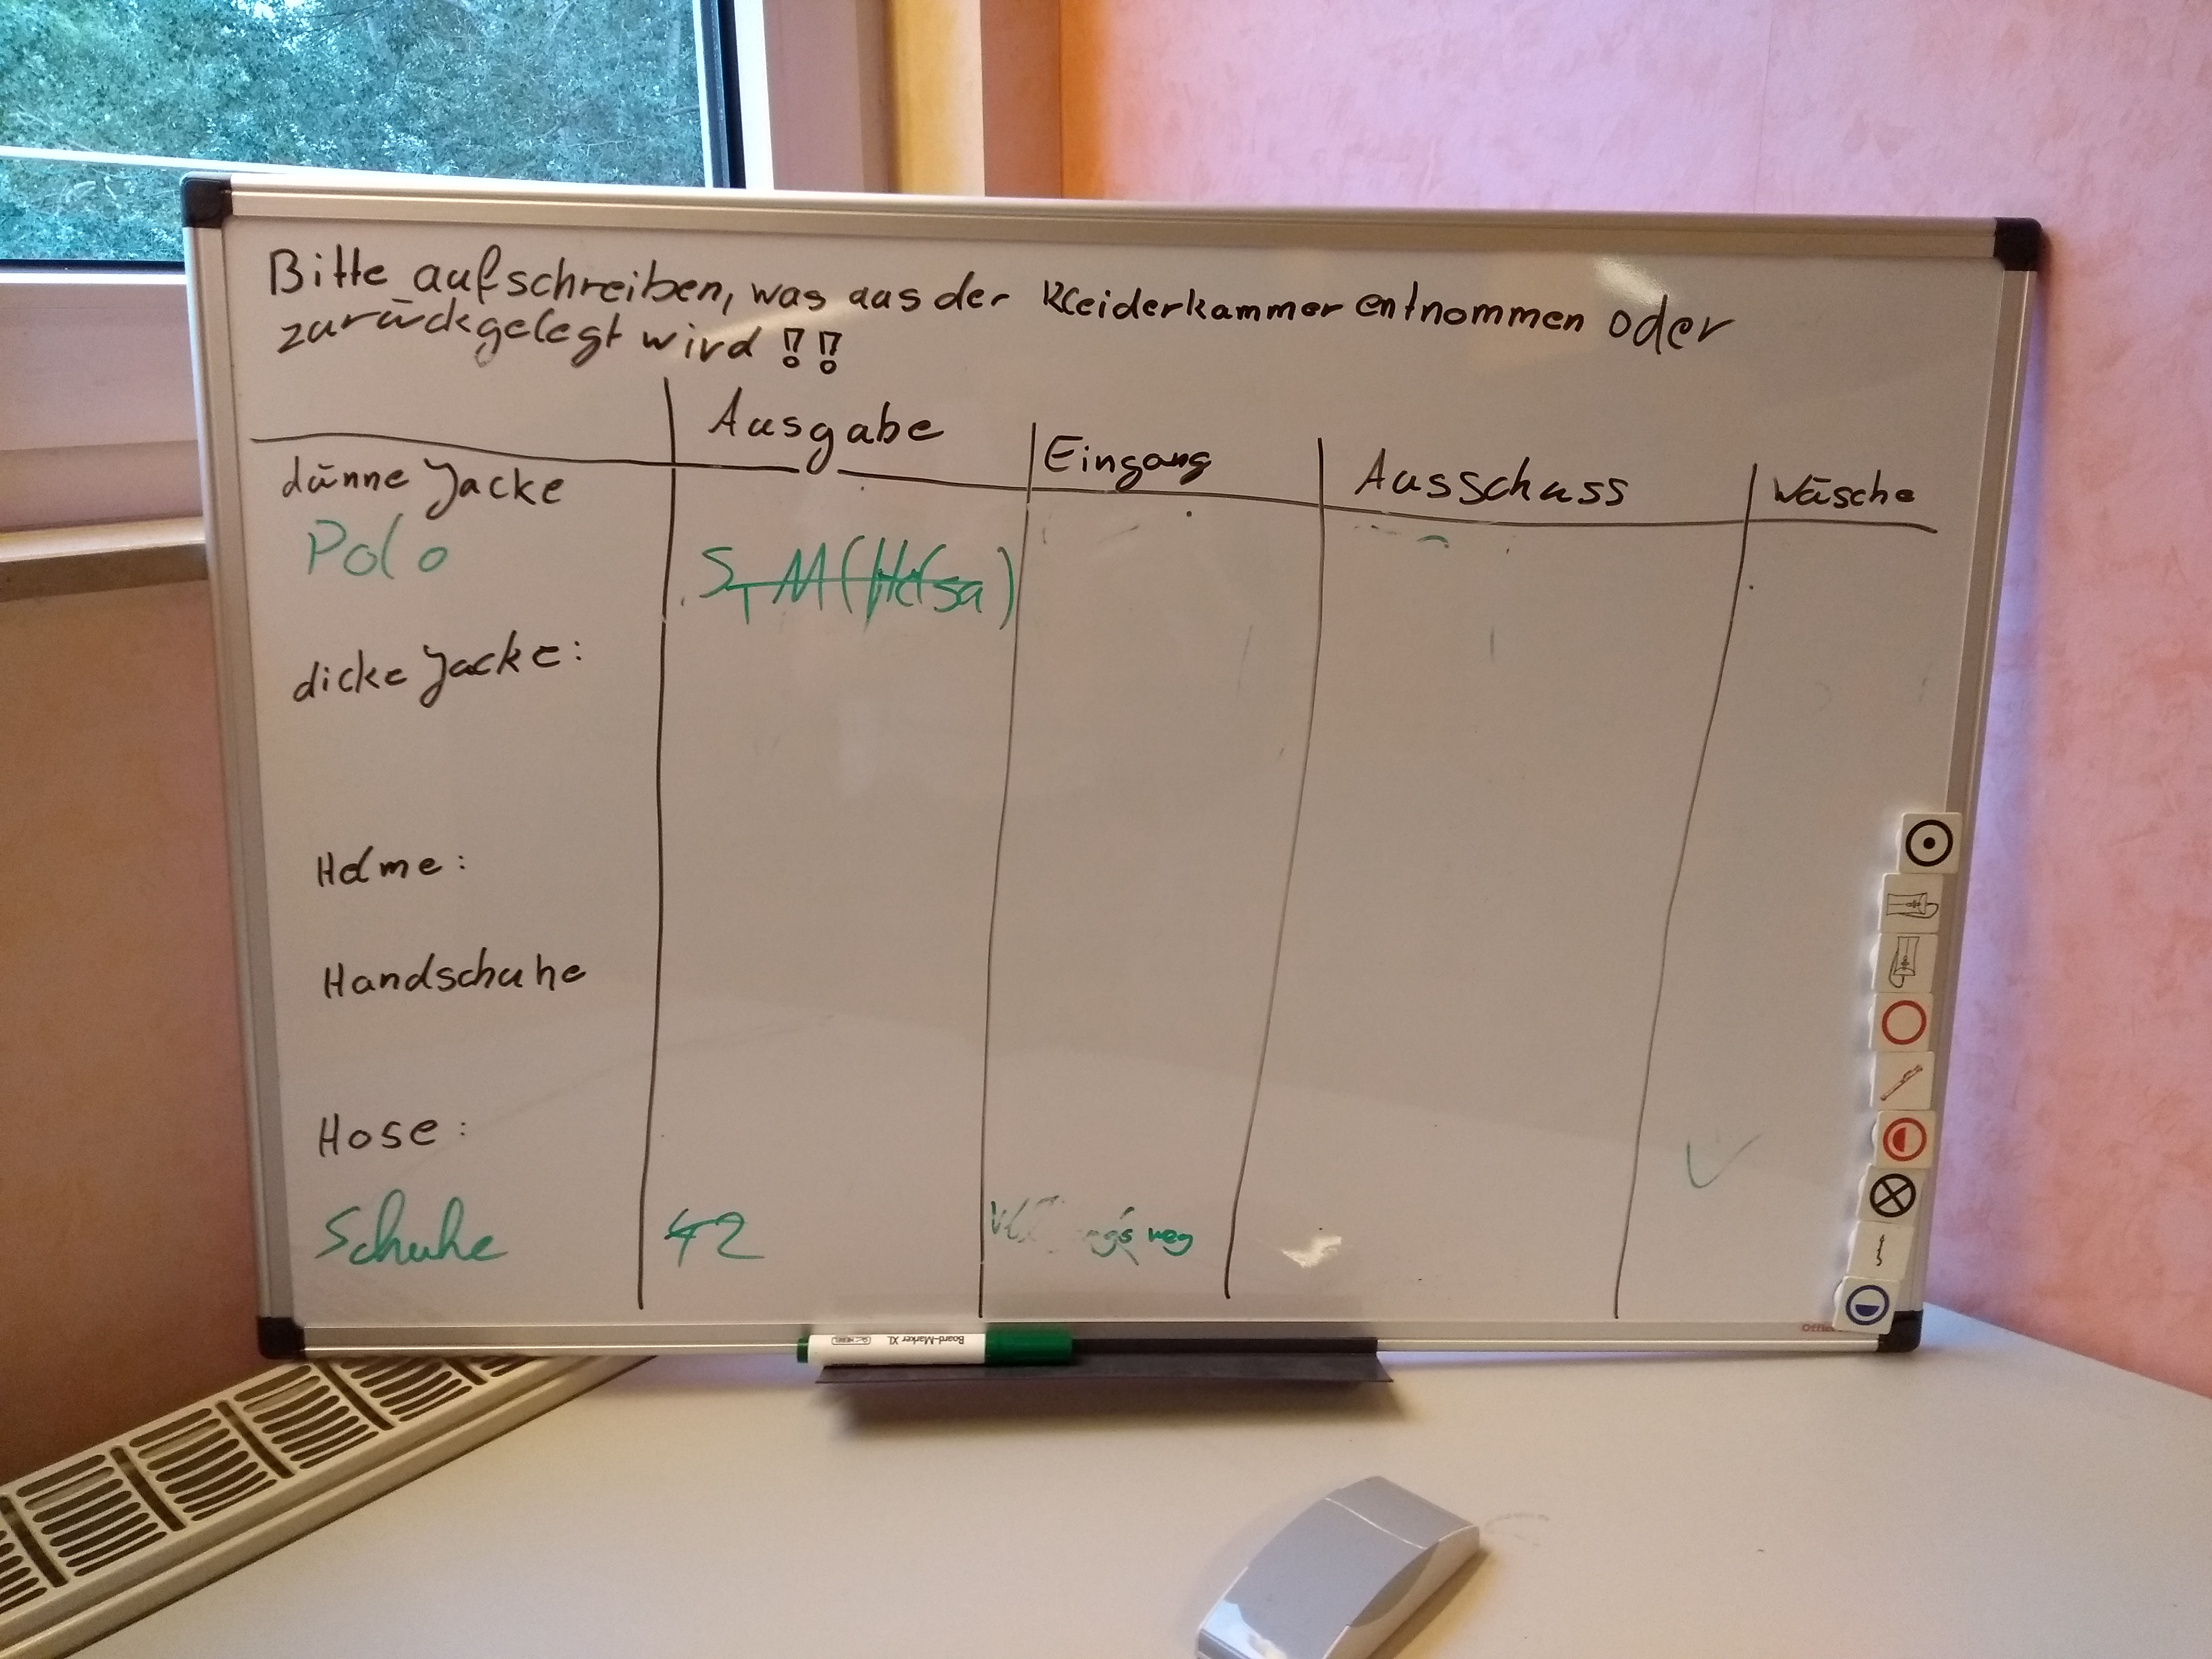
\includegraphics[width=0.95\textwidth]{res/IMG_20180815_193814370}
  \caption{Tafel aus Zwischenspeicher von Informationen.}
  \label{fig:tafel}
\end{figure}

Um die Probleme des Datenverlusts und der Synchronisation von Daten zu beseitigen, kam die Idee einer zentralen, aus dem Internet erreichbaren Kleiderverwaltung der Jugendfeuerwehr von Eschenstruth, oder auch \project, auf.

In den folgenden Kapiteln werden die Kernziele dieses Projekts erläutert und die Erfolgskriterien definiert. Die beteiligten Personen an diesen Projekt werden erfasst und kurz vorgestellt. Darauf folgt der Projektansatz mit der Anforderungsspezifikation. Dabei werden alle Anforderungen die zwingend in diesem Projekt umgesetzt werden müssen definiert. 

\subsection{Project Definition Document}

\subsubsection{Gegenstand, Kernziele und Ziele des Projektes}

Unsere Kernziele sind das Schaffen einer Übersicht über die Bestände der Kleidung der Jugendfeuerwehren der Gemeinde Helsa. Diese werden aktuell im Ortsteil Eschenstruth gelagert und rudimentär verwaltet. Dafür soll eine Web"=Applikation erstellt werden, die den Bestand dokumentiert, die Auf"= und Abgabe von Kleidung der freiwilligen Feuerwehr Helsa Ortsteil Eschenstruth ermöglicht. 

Das Projekt soll möglichst barrierefrei (nach aktuellstem europäischem Standard), sowie mobil bedienbar sein, sodass die Jugendwarte nicht auf einen zusätzlichen Laptop angewiesen sind, sondern das Programm einfach und bequem von ihrem Handy oder Smartphone aus bedienen können. Es soll außerdem unter Verwendung der aktuellsten technischen Standards umgesetzt werden.

Ziel ist es eine vollständig nachvollziehbare Dokumentation zu ermöglichen, bei dem zu jederzeit der aktuelle Aufenthaltsort der zur Verfügung stehenden Kleidung ermittelt werden kann. Dabei soll ein paralleles Arbeiten möglich sein. 

\subsubsection{Erfolgskriterien}

Wir sind sehr darauf bedacht, dass unsere Anwendung performant läuft und jederzeit erreichbar ist. Hierfür ist uns eine gute Server-Infrastruktur wichtig. Dass unsere Applikation performant ist, ist uns wichtig, da es die Akzeptanz unserer Anwender steigern wird, wenn sie nicht lange auf einen Seitenaufbau oder auf das Ausführen einer Aktion warten müssen. 

Wie legen außerdem gesteigerten Wert darauf, dass die Anwendung mobil nutzbar sein wird. Das soll zum einen ebenfalls die Akzeptanz der Anwender steigern und zum anderen das Anschaffen neuer Hardware verhindern.

Ein weiteres Erfolgskriterium ist die vollständige Ablösung der Excel"=Tabelle und der Tafel. Die Daten werden nur noch über die Anwendung gepflegt.

\subsubsection{Kontext des Projektes und die Projektabhängigkeiten}

Unser Projekt wird im Kontext unseres Studiums der Sozialinformatik umgesetzt. 

Das Projekt soll für einen öffentlichen, sozialen Träger umgesetzt werden: Die freiwillige Feuerwehr der Gemeinde Helsa, oder spezifisch des Ortsteiles Eschenstruth. Dort sind nur ehrenamtliche Kräfte tätig, die für den Brandschutz in der Gemeinde Helsa und den neuen Autobahnabschnitt der A44 zwischen Kassel und Hessisch-Lichtenau Sorge tragen und gewährleisten. 

\subsubsection{Risiken, die den Projekterfolg verhindern könnten}

Dadurch, dass das Projekt"=Team Vollzeit tätig ist, kann es zu Engpässen in der Durchführung kommen. Dies kann unter Umständen zu Mehrarbeit auf einzelne Team"=Mitglieder führen. Das Risiko ist gering einzuschätzen, da das Projekt"=Team  hinter der Idee steht.

Ein weiteres Risiko betrifft die Evaluation einer kostenlosen, bis kostengünstigen, Plattform, auf der die Anwendung bereit gestellt werden kann. Dabei kann die Akzeptanz der Endkunden sinken, wenn die Betriebskosten zu hoch ausfallen. Ab welchen Betrag die Kosten zu hoch sind, ist noch zu klären. Dieses Risiko ist mittelmäßig einzuschätzen, da es am Markt diverse Anbieter gibt. Unter den bekannteren Anbietern gehören \textit{AWS}, von \textit{Amazon}, und \textit{Heroku}.

\subsubsection{Am Projekt Beteiligte}\label{sec:beteiligte}

Zum Projekt"=Team gehören:

\begin{itemize}
\item Tim Wieder, ist zuständig für den Kundenkontakt und die Frontend"=Entwicklung.
\item Achim Rose, ist zuständig für die Backend"=Entwicklung und den Entwurf der Datenbanktabellen. 
\item Sebastian Seeger, ist zuständig für die Infrastruktur. Das betrifft die Evaluation der Plattform und dessen Konfiguration.
\end{itemize}

Zu den Kunden, sprich die Beteiligten der freiwilligen Feuerwehr Eschenstruth, gehören: 

\begin{itemize}
\item Nico M. (zuständig für die Kleiderkammer)
\item Julia W.
\item Marcel B.
\item Markus N.
\item Florian B.
\item Philipp H.
\end{itemize}

\subsubsection{Zu erwartender Projektansatz}

Das Projekt wird mit dem agilen Softwareentwicklungsframework \textit{Scrum} umgesetzt. Der Vorteil hierbei ist die Freiheit für die Entwickler, die sich die Arbeit so einteilen können, wie es für sie gerade passend ist. Dabei werden regelmäßig Dailys abgehalten, um die anderen Projektteilnehmer auf den aktuellen Entwicklungsstand zu bringen.

\newpage

\section{Projektplanung}\label{sec:Projektplanung}

Diese Anforderungsspezifikation ist die Aufnahme der Bedürfnisse nach dem ersten Meeting mit den Stakeholdern. Durch die Verwendung von \textit{Scrum} können wir durch die grobe Beschreibung der Anforderungen unsere Sprints planen und bei der Erstellung der Datenbankstruktur auf die Anforderungen zurück greifen. 

\subsection{Anforderungsspezifikation}

Die Anwendung wird in vier Abschnitte gegliedert: Startseite, Aktionen, Auswertungen und Administration.

Auf der \textit{\textbf{Startseite}} müssen die letzten 20 Transaktionen aufgelistet werden. Dabei werden die Informationen über die Transaktion selbst angezeigt, sowie die Person die die Transaktion ausgeführt hat.

Die Transaktionen, oder auch Aktionen, werden im Abschnitt \textit{\textbf{Aktionen}} durchgeführt. Eine Transaktion umschließt die Informationen der \textit{Kleidungsart}, \textit{Stückzahl}, \textit{Größe}, \textit{Bestimmungsort}, \textit{Art der Aktion} und der \textit{ausführenden Person}. Bei einer Transaktion müssen immer die Informationen über die Kleidungsart, die Stückzahl, die Größe und den Bestimmungsort angegeben werden. Dabei werden Kleidungsart, Größe und Stückzahl in einer Gruppe erfasst damit mehrere Kleidungsarten in einer Transaktion an einen Bestimmungsort übergeben werden können. 

Über die Art der Aktion können der Anwender*innen festgelegen, ob die Kleidungsstücke an einen Bestimmungsort \textit{ausgegeben}, \textit{zurückgenommen} oder \textit{ausgesondert} werden. Kleidungsstücke können auch in die Wäsche gegeben werden. Dies ist notwendig um den Überblick über den Bestand zu wahren und nicht bei Mangel während der Ausgabe die Notwendigkeit zu sehen, Kleidungsstücke zu bestellen.

Der \textit{Bestimmungsort} kann ein Ortsteil der Feuerwehr sein oder das Lager, \bzw der Wareneingang. Somit lässt sich erkennen, ob Kleidungsstücke in den Warenbestand aufgenommen wurden, oder an einen Ortsteil ausgegeben wurde.
Aus den Aktionen resultiert für die Startseite die Liste der Transaktion in natürlich sprachlichen Texten. Zum Beispiel: 
\begin{itemize}
\item 5 dünne Jacken in Größe 40 vom Ortsteil Helsa ausgesondert, durch Max Mustermann am 14.12.2019 09:43 Uhr.
\item 12 Hosen in Größe 32 ins Lager aufgenommen, durch Max Mustermann am 10.12.2019 15:26 Uhr.
\item 12 Hosen in Größe 32 vom Lager in der Wäsche, durch Max Mustermann am 10.12.2019 12:02 Uhr.
\item 10 Jacken in Größe 40, 10 Stiefel in Größe 36 vom Ortsteil Helsa ausgegeben, durch Max Mustermann am 06.12.2019 18:12 Uhr.
\item 10 Jacken in Größe 40, 10 Stiefel in Größe 36 vom Wareneingang aufgenommen, durch Max Mustermann am 05.12.2019 17:30 Uhr.
\end{itemize}

Die Kleidungsstücke und deren Größen, sowie die Ortsteile und die Anwender*innen, können in der \textbf{\textit{Administration}} verwaltet werden.

In der Administration der Ortsteile können beliebige Ortsteile nach Bedarf hinzugefügt werden. Dabei muss der Name angegeben werden und ein Ansprechpartner. Optional können weitere Ansprechpartner zu einem Ortsteil hinzufügt oder bis auf einen entfernt werden. Ein Ortsteil kann auch inaktiv gesetzt werden. Hierbei muss jedoch geprüft werden, ob sich noch Kleidungsstücke auf den Ortsteil gebucht sind. Das Inaktiv setzen ist erst dann möglich, wenn alle Kleidungsstücke in den Warenbestand zurück gebucht wurden. Es bietet sich an, dafür eine Komfort"=Funktion bereit zu stellen. Diese Transaktion muss auch über die Startseite erkennbar sein. Ein Ortsteil kann deshalb nicht gelöscht werden, weil durch den Verlust der Information die Transaktionen nicht mehr vollständig nachvollziehbar wären. Ein Ortsteil kann nur dann effektiv gelöscht werden, wenn keinerlei Transaktionen darauf ausgeführt wurden.

Am Ortsteil können Grenzen der Anzahl von Kleidungsstücken bestimmt werden, bei dem eine Warnung erscheint, wenn zu viele Kleidungsstücke ausgegeben wurden. Diese Warnung erscheint bei den Aktionen nach der Auswahl des Ortsteils. Wenn keine Grenze angegeben wurde, wird nichts geprüft.

Ein weiterer Punkt der Administration ist die Benutzerverwaltung. Hier können Personen angelegt und gelöscht, ihre Rechte verwaltet und der Einkäufer bestimmt werden. Dazu müssen der Name, die E"=Mail Adresse gespeichert werden. Zudem kann gesteuert werden, ob die Person nur lesenden, schreibenden oder administrativen Zugriff auf das System hat. Bei lesendem Zugriff ist die Seite der Aktionen gesperrt. Bei schreibenden Zugriff ist die Seite der Administration gesperrt. Der Administrator hat auf alle Bereiche Zugriff. Die Einstellung, ob eine Person für den Einkauf zuständig ist, ist mit der Administration der Kleidungsstücke verknüpft. 

Die Kleidungsarten und die dazugehörigen Größen können in der Administration erweitert werden. Diese können nur gelöscht werden, wenn noch keine Transaktionen mit der Kleidungsart und Größe vorgenommen wurde. Dies ist besonders wichtig, damit die Auswertungen auch weiterhin nachvollziehbar und reproduzierbar sind. Kleidungsarten können aber inaktiv gesetzt werden, wodurch diese bei Aktionen nicht mehr ausgewählt werden können. Zu jeder Kombination von Kleidungsart und Größe kann ein Grenzwert festgelegt werden, bei dem die Einkäufer*innen eine E"=Mail Benachrichtigung erhalten. Damit diese Grenze nicht bei jeder Neuanlage eingetippt werden muss, kann der Standardwert angegeben werden.

Im Abschnitt der \textit{\textbf{Auswertungen}} können die Anwender*innen eine Bericht erstellen, der Auskunft über die ausgegebenen, zurückgenommenen und ausgesonderten Kleidungsstücke gibt. Dabei kann in einem Filter der Zeitraum, die Kleidungsart, Größe, Transaktionsart, der Ortsteil (wie auch der lokale Warenbestand) gesetzt werden, wodurch der Bericht auf spezielle Bedürfnisse angepasst werden kann. Der Bericht soll als Excel"=Tabelle oder PDF erfolgen.

\subsection{Projektplan}
\subsubsection{Work-Breakdown-Structure}\label{sec:wbs}

\textit{TODO: Verschriftlichen}

\begin{itemize}
\item Phase 1 (Aug-Sept 2018)
  \begin{itemize}
  \item Get in contact with stakeholders
  \item Analyse and document requirements (upcoming data / rest-services / security)
  \item Design frontend/backend architecture and server infrastructure
  \item Setup project structure with https://start.spring.io/
  \item Setting up Continious Integration (build/release process). Goal: build and release pipeline. (Jenkins? Nexus? Maven Repo?)
  \item Project-Init (documents output)
  \item Project definition document
  \item Project plan
  \end{itemize}

\item Phase 2 (Feb-Mar 2019)
  \begin{itemize}
  \item Define definition of done (DOD).
  \item Iterative sprints (1 week) with daylies (10 minutes via Skype)
  \item Developing backend / frontend. Setup, configure, maintanance database / server.
  \item Documentation and tests
  \item Full Agile and so. Tim will know (at least scrum master, haha)
  \item document output
  \item project diary
  \end{itemize}

\item Phase 3 (Aug-Sept 2019)
  \begin{itemize}
  \item Same as phase 2 :
  \end{itemize}

\item Phase 4 (Feb-Mar 2020)
  \begin{itemize}
  \item project closure
  \end{itemize}
\end{itemize}

\subsubsection{Ressourcenplanung}

Kann schon geplant werden, wer für welche Aufgabe zuständig ist? Dann eine Tabelle mit der Resourcenplanung erstellen.


\subsubsection{Zeitplanung}

Hier noch ein Gantt. Als Bild...

% falls man lieber eine Datei pro Kapitel bevorzug, kann man dies auch einfach realisieren, indem man diese wie folgt einbindet
%\input{src/kapitel01.tex}
%\input{src/kapitel02.tex}
%\input{src/kapitel03.tex}
% diese müssen dann natürlcih in dem Ordner vorliegen


%\newpage

%\section{Absicherung des Systems}\label{sec:Security}

Da es sich bei der Kleiderverwaltung um ein geschlossenen System handelt, dass nur von einem bestimmten Personenkreis verwendet werden darf, muss die Person sich authentifizieren. Das System prüft die Anmeldedaten und autorisiert die Person, wenn seine Anmeldedaten korrekt sind und sie im System als Benutzer*in hinterlegt ist.

Wie die Registrierung und Anmeldung genau funktionieren soll, wird in den folgenden Kapitel genauer beschrieben.

\subsection{Registrierung}



\subsection{Anmeldung}

Damit nur berechtigte Personen Zugriff auf das System erhalten, muss die Anwendung abgesichert werden. Die Authentifizierung geschieht im Backend. Im öffentlichen Zugriff steht nur die Anmeldung. Im abgesicherten Bereich können nur angemeldete Personen Daten lesen und schreiben. Über die erfolgreiche Anmeldung am Backend wird der Person ein Json Web Token (JWT) geliefert, das im Header \textit{Authorization} bei jedem HTTP-Request mitgegeben werden muss. Das Token beinhaltet den Nutzernamen und die Dauer bis wann die Anmeldung gültig ist. 

Anmeldung: Ein Token wird erzeugt, an den Client zurückgegeben.
Bei einem Request: Token auffrischen, sofern bereits ein Token besteht.
Abmelden: Token aus der DB löschen.

Damit angemeldete Personen sich Abmelden können, werden die Token mit in der Datenbank gespeichert. Bei der Abmeldung wird der Token aus der Benutzertabelle entfernt. Dadurch muss ein neues Token erzeugt werden.

\textit{Ablaufplan?}

\textit{Was ist das JWT?}



\newpage

% nocite lässt alle Werke anzeigen, auch solche die nicht verlinkt sind. 
%\nocite{*}
\printbibliography[heading=head]

\newpage

% Rudi will kein Abbildungsverzeichnis
\listoffigures
\addcontentsline{toc}{section}{\listfigurename}

\listoftables
\addcontentsline{toc}{section}{Tabellenverzeichnis}

%\lstlistoflistings
%\addcontentsline{toc}{section}{Listings}

\newpage


%%!TEX root = ../hausarbeit.tex
% Erklaerung der Selbststaendigkeit.
% Footer wird in config.tex durch \AtEndDocument{\ofoot{}} angepasst
\section*{Erklärung der Selbständigkeit}
\addcontentsline{toc}{section}{Erklärung der Selbständigkeit}
Ich versichere, dass ich die vorliegende schriftliche Prüfungsleistung selbständig verfasst, keine anderen als die angegebenen Quellen und Hilfsmittel verwendet habe und die Stellen, die anderen Werken im Wortlaut oder dem Sinn nach entnommen sind, im Text jeweils mit Quellenbelegen kenntlich gemacht habe. Die Arbeit ist noch nicht anderweitig für Prüfungszwecke vorgelegt worden.
\\
\\
\\
\\
\\

\parbox{5cm}{\centering  \ortderarbeit, \today\hrule\strut\centering\footnotesize Ort, Datum}
\hfill
\vspace{-2cm}
\parbox{6cm}{\centering {\color{white} X} \hrule\strut \centering\footnotesize Unterschrift}
%\vspace{-2cm} %hochschieben
%\includegraphics[width=0.4\textwidth,heigth=12pt]{res/Unterschrift.png}
%\vspace{2cm} % wieder runter


\end{document}

